\documentclass{article}
% generated by Madoko, version 1.1.3
%mdk-data-line={1}


\usepackage[heading-base={2},section-num={False},bib-label={hide},fontspec={True}]{madoko2}


\begin{document}



%mdk-data-line={6}
\mdxtitleblockstart{}
%mdk-data-line={6}
\mdxtitle{\mdline{6}PhxQueue调研及测试报告}%mdk
\mdxauthorstart{}
%mdk-data-line={11}
\mdxauthorname{\mdline{11}ryanyycao(曹洋毓)}%mdk
\mdxauthorend\mdtitleauthorrunning{}{}\mdxtitleblockend%mdk

%mdk-data-line={8}
\section{\mdline{8}1.\hspace*{0.5em}\mdline{8}PhxQueue综述}\label{sec-phxqueue}%mdk%mdk

%mdk-data-line={10}
\noindent\mdline{10}\hspace*{1em}\mdline{10}\hspace*{1em}\mdline{10}PhxQueue是一款基于Paxos协议实现的高可用、高吞吐、高可靠的分布式队列,保证At-Least-Once Delivery。%mdk

%mdk-data-line={12}
\mdline{12}\hspace*{1em}\mdline{12}\hspace*{1em}\mdline{12}PhxQueue支持的主要特性有同步刷盘,出入队严格有序,多订阅,出队限速,出队重放,所有模块均可平行扩展,存储层批量刷盘、同步,保证高吞吐,存储层支持同城多中心部署,存储层自动容灾/接入均衡,消费者自动容灾/负载均衡等。%mdk

%mdk-data-line={14}
\section{\mdline{14}2.\hspace*{0.5em}\mdline{14}PhxQueue系统设计}\label{sec-phxqueue}%mdk%mdk

%mdk-data-line={16}
\begin{itemize}[noitemsep,topsep=\mdcompacttopsep]%mdk

%mdk-data-line={16}
\item\mdline{16}\textbf{整体结构}\mdline{16}%mdk
%mdk
\end{itemize}%mdk

%mdk-data-line={18}
\noindent\mdline{18}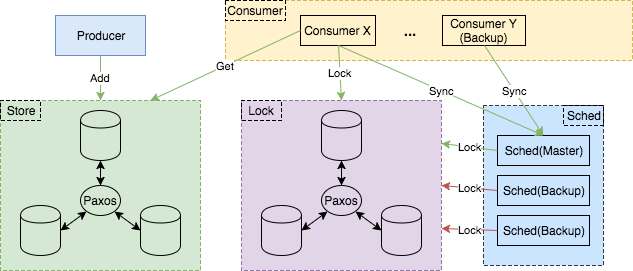
\includegraphics[keepaspectratio=true,width=\dimmin{}{\dimwidth{0.90}}]{images/1505466623_80_w633_h271}{}\mdline{18}%mdk

%mdk-data-line={23}
\begin{itemize}%mdk

%mdk-data-line={23}
\item{}
%mdk-data-line={23}
\mdline{23}\textbf{Store - 队列存储}\mdline{23}%mdk

%mdk-data-line={25}
\mdline{25}  \mdline{25}\hspace*{1em}\mdline{25}\hspace*{1em}\mdline{25}Store 作为队列存储,引入了PhxPaxos库,以Paxos协议做副本同步,副本数为3,三副本状态强一致,免去了去重逻辑。只要多数派节点正常工作及互联,即可提供线性一致性读写服务。为了提高数据可靠性,同步刷盘作为默认开启特性,且性能不亚于异步刷盘。在可用性方面,Store 内有多个独立的 paxos group,每个 paxos group仅master提供读写服务,平时master动态均匀分布在Store内各节点,均衡接入压力,节点出灾时自动切换master到其它可用节点。
\mdline{26}\mdbr
\mdline{27}  \mdline{27}\hspace*{1em}\mdline{27}\hspace*{1em}\mdline{27}Store使用状态机完成复制,各节点在状态机只保存索引,而不保存队列数据,需要读取队列数据时直接访问plog,这种特性可以在积压下让存储成本减半,同时写带宽减半。
\mdline{28}\mdbr
\mdline{29}  \mdline{29}\hspace*{1em}\mdline{29}\hspace*{1em}\mdline{29}Store同步刷盘带来写放大,采用多 paxos group 部署 以及 Group Commit 的方式来同时解决同步刷盘的写放大问题以及Paxos吞吐问题。优势:业务层无需关注如何组织请求进行批量;在存储层以 paxos group 为单位的聚合效果比上层聚合效果更好。
\mdline{30} \mdline{30}%mdk%mdk

%mdk-data-line={32}
\item{}
%mdk-data-line={32}
\mdline{32}\textbf{Producer - 生产者}\mdline{32}%mdk

%mdk-data-line={34}
\mdline{34}  \mdline{34}\hspace*{1em}\mdline{34}\hspace*{1em}\mdline{34}Producer 作为消息生产者,根据key决定消息存储路由。相同key的消息默认路由到同一个队列中,保证出队顺序与入队顺序一致。%mdk%mdk

%mdk-data-line={36}
\item{}
%mdk-data-line={36}
\mdline{36}\textbf{Consumer - 消费者}\mdline{36}%mdk

%mdk-data-line={38}
\mdline{38}  \mdline{38}\hspace*{1em}\mdline{38}\hspace*{1em}\mdline{38}Consumer 作为消费者,以批量拉取的方式从Store拉消息,支持多协程方式批量处理消息。Consumer以服务框架的形式提供服务,使用者以实现回调的方式,根据不同主题(Topic),不同处理类(Handler)定义具体的消息处理逻辑。%mdk%mdk

%mdk-data-line={40}
\item{}
%mdk-data-line={40}
\mdline{40}\textbf{Scheduler - 消费者管理器}\mdline{40}%mdk

%mdk-data-line={42}
\mdline{42}  \mdline{42}\hspace*{1em}\mdline{42}\hspace*{1em}\mdline{42}Scheduler 的作用是, 对 Consumer 做容灾(通过心跳定义Consumer生死)和负载均衡(收集 Consumer 全局负载信息)。当使用者没有这方面的需求时,可以省略部署 Scheduler,此时各 Consumer 根据配置权重决定与队列的处理关系。
\mdline{43}\mdbr
\mdline{44}  \mdline{44}\hspace*{1em}\mdline{44}\hspace*{1em}\mdline{44}负载均衡器采用master单点服务的模式, 自然实现强一致。master依赖分布式锁选举,master挂了可自行切换。在master的failover期间,仅消费者的自动容灾和负载均衡逻辑失效,出入队不受影响,也就是说整个队列系统不对负载均衡器强依赖。%mdk%mdk

%mdk-data-line={46}
\item{}
%mdk-data-line={46}
\mdline{46}\textbf{Lock - 分布式锁}\mdline{46}%mdk

%mdk-data-line={48}
\mdline{48}  \mdline{48}\hspace*{1em}\mdline{48}\hspace*{1em}\mdline{48} Lock 引入Paxos提供通用分布式锁服务,可以独立部署。在PhxQueue中的作用有两点,为 Scheduler 选举 leader,防止多个 Consumer 同时处理一条队列。%mdk%mdk
%mdk
\end{itemize}%mdk

%mdk-data-line={50}
\section{\mdline{50}3.\hspace*{0.5em}\mdline{50}PhxQueue VS Kafka}\label{sec-phxqueue-vs-kafka}%mdk%mdk

%mdk-data-line={52}
\subsection{\mdline{52}3.1.\hspace*{0.5em}\mdline{52}设计对比}\label{section}%mdk%mdk

%mdk-data-line={54}
\noindent\mdline{54}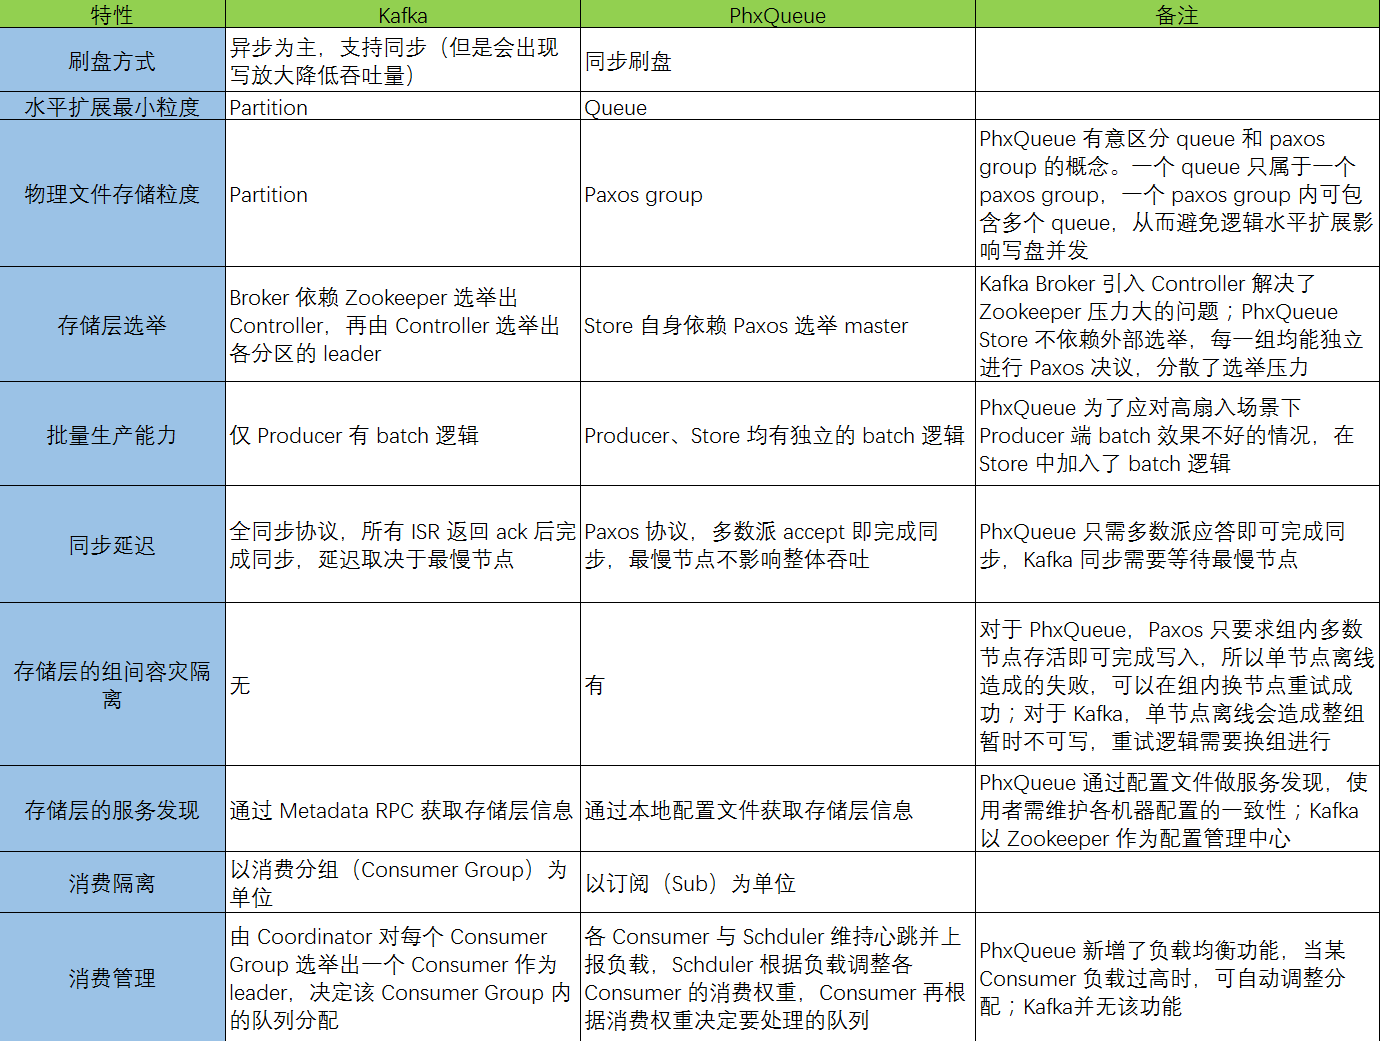
\includegraphics[keepaspectratio=true,width=\dimmin{}{\dimwidth{0.90}}]{images/-96D645D6-2667-48C2-AE3E-4102FEB3EC8D-}{}\mdline{54}%mdk

%mdk-data-line={60}
\subsection{\mdline{60}3.2.\hspace*{0.5em}\mdline{60}性能对比}\label{section}%mdk%mdk

%mdk-data-line={62}
\begin{itemize}[noitemsep,topsep=\mdcompacttopsep]%mdk

%mdk-data-line={62}
\item\mdline{62}\textbf{测试环境}\mdline{62}:b70\mdline{62}*\mdline{62}3%mdk
%mdk
\end{itemize}%mdk

%mdk-data-line={64}
\noindent\mdline{64}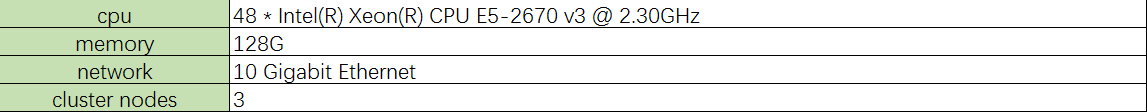
\includegraphics[keepaspectratio=true,width=\dimmin{}{\dimwidth{0.90}}]{images/-2709511A-3B33-40CE-A125-DDFAD9C0FF2F-}{}\mdline{64}%mdk

%mdk-data-line={68}
\begin{itemize}%mdk

%mdk-data-line={68}
\item{}
%mdk-data-line={68}
\mdline{68}\textbf{测试结果}\mdline{68}:默认的kafka配置,qps为13万/秒,平均延迟为230ms;PhxQueue吞吐远低于kafka,qps取决于磁盘IOPS。\mdline{68}\mdbr
\mdline{69}(原因:由于kafka在写盘时用到了Memory Mapped Files技术,这种技术支持内存映射文件,所以在写盘时其实是写入内存,之后再批量写入硬盘,省去了磁盘读写的时间;而由于PhxQueue没有做wal,所以其每次存储都得单独执行一次磁盘存储,试验采用的是sata磁盘机器,严重影响了qps,想要压测出PhxQueue的极限吞吐需要使用ssd的机器。官方给出ssd下PhxQueue吞吐还要略高于Kafka)%mdk%mdk

%mdk-data-line={71}
\item{}
%mdk-data-line={71}
\mdline{71}\textbf{结论}\mdline{71}:在sata磁盘环境下,kafka吞吐远超PhxQueue,但是PhxQueue设计的优势在于其在高扇入同步刷盘场景下的使用,可靠性更强,在使用ssd以后吞吐和kafka不相上下(官方数据)。对于压测瓶颈,若使用ssd,PhxQueue 瓶颈在 cpu,大概在70\%,若使用sata,PhxQueue 瓶颈在磁盘读写,Kafka 瓶颈通常都在磁盘读写。%mdk%mdk
%mdk
\end{itemize}%mdk

%mdk-data-line={73}
\subsection{\mdline{73}3.3.\hspace*{0.5em}\mdline{73}存储层 failover 过程对比}\label{sec--failover-}%mdk%mdk

%mdk-data-line={75}
\begin{itemize}[noitemsep,topsep=\mdcompacttopsep]%mdk

%mdk-data-line={75}
\item\mdline{75}\textbf{Kafka}\mdline{75}:Failover 期间,在不同阶段程度不同,入队成功率在0\% \mdline{75}\textasciitilde{}\mdline{75} 33\%;Failover 持续时间由租约决定,租约时长默认10s。%mdk

%mdk-data-line={76}
\item\mdline{76}\textbf{PhxQueue}\mdline{76}:Failover 期间,入队成功率仅下降至66\%;Failover 持续时间由租约决定,租约时长默认5s;开启换队列重试特性(适合没有绝对顺序性要求的业务提高可用性)后,Failover 期间仍有90+\%入队成功率。%mdk
%mdk
\end{itemize}%mdk

%mdk-data-line={78}
\subsection{\mdline{78}3.4.\hspace*{0.5em}\mdline{78}API}\label{sec-api}%mdk%mdk

%mdk-data-line={80}
\begin{itemize}%mdk

%mdk-data-line={80}
\item{}
%mdk-data-line={80}
\mdline{80}\textbf{Kafka}\mdline{80}:主要包括五种API:\mdline{80} \mdline{80}%mdk

%mdk-data-line={82}
\mdline{82}\textbf{Producer API}\mdline{82}:允许应用程序将数据流发送的集群中的topics\mdline{82}\mdbr
\mdline{83}\textbf{Consumer API}\mdline{83}:允许应用程序从集群的topics中读出数据流\mdline{83}\mdbr
\mdline{84}\textbf{Streams API}\mdline{84}:允许将数据流从input topics传输到output topics\mdline{84}\mdbr
\mdline{85}\textbf{Connect API}\mdline{85}:允许实现一些连接器,可以连续的从其他源系统或者应用程序拉取数据到kafka,或者将kafka数据图推送到其他系统或应用程序\mdline{85}\mdbr
\mdline{86}\textbf{AdminClient API}\mdline{86}:允许管理和检查topics,brokers和一些其他的kafka组件\mdline{86} \mdline{86}%mdk%mdk

%mdk-data-line={88}
\item{}
%mdk-data-line={88}
\mdline{88}\textbf{Phxqueue}\mdline{88}:bg内部有搭好的云服务,可以直接从运维系统接入,不需要管理,主要包括三种API:\mdline{88} \mdline{88}%mdk

%mdk-data-line={90}
\mdline{90}\textbf{发布者}\mdline{90}:使用svrkit协议,运维分配一个evcpubid,每套事件中心有独立的Api, 调用方式一致,只是类名不一样,具体接入时提供,调用Public接口发布消息,事务调用Commit/RollBack接口来确认发送或者回退消息\mdline{90}\mdbr
\mdline{91}\textbf{订阅者}\mdline{91}:可以使用http协议(普通的httpsvr和logicsvr)或svrkit协议\mdline{91}\mdbr
\mdline{92}\textbf{反查}\mdline{92}:可以使用http协议(普通的httpsvr和logicsvr)或svrkit协议\mdline{92} \mdline{92}%mdk%mdk
%mdk
\end{itemize}%mdk

%mdk-data-line={95}
\section{\mdline{95}4.\hspace*{0.5em}\mdline{95}总结}\label{section}%mdk%mdk

%mdk-data-line={98}
\noindent\mdline{98}\hspace*{1em}\mdline{98}\hspace*{1em}\mdline{98}PhxQueue 是一款基于Paxos协议实现的高可用、高吞吐、高可靠的分布式队列,并且做了很多的优化:支持同步刷盘,保证了同步刷盘的吞吐,其性能不亚于异步刷盘;在Store端做了batch逻辑,解决了高扇入场景Producer端batch效果不好的问题,解决了写放大的问题;同步延迟只需多数派应答,响应更快;做了负载均衡的特性,自动调整Consumer负载;稳定性更强,在节点失效时成功率影响不大。更加是用于不能做batch,需要同步刷盘,保证可靠性的业务场景%mdk

%mdk-data-line={100}
\mdline{100}\hspace*{1em}\mdline{100}\hspace*{1em}\mdline{100}Kafka 设计的目标则是高吞吐量、低延迟的消息系统,将消息作为文件来处理,无论是写入数据和写出数据吞吐量都很大,更适用于不要求同步刷盘的应用场景。%mdk

%mdk-data-line={103}
\begin{mdbmargintb}{4em}{}%mdk
\begin{mdflushright}%mdk
{\tiny\mdline{104}Created with~\href{https://www.madoko.net}{Madoko.net}.}%mdk
\end{mdflushright}%mdk
\end{mdbmargintb}%mdk%mdk


\end{document}
